% Masterthesis talk
% Multiscale Modelling Group of Jun.-Prof. Birgit Strodel
% Given on November 04, 2013 at FZ Juelich
%
% Oliver Schillinger

\documentclass[english]{beamer}

\usetheme{Juelich}
\usepackage[scaled]{helvet}

\usepackage[british]{babel}
\usepackage{graphicx,hyperref,url,color}
\usepackage{amsmath}
\usepackage[latin1]{inputenc}
\usepackage[T1]{fontenc} 

\usepackage{ulem}

\setbeamertemplate{slide counter}[showall][]

\hypersetup{
    %bookmarks=false,        % show bookmarks bar?
    unicode=false,          % non-Latin characters in Acrobat’s bookmarks
    pdftoolbar=true,        % show Acrobat’s toolbar?
    pdfmenubar=true,        % show Acrobat’s menu?
    pdffitwindow=false,     % window fit to page when opened
    pdfstartview={FitH},    % fits the width of the page to the window
    pdftitle={Talk Masterthesis},    % title
    pdfauthor={Oliver Schillinger},     % author
    pdfsubject={Structure of Lipase-CitAP complex},   % subject of the document
    pdfcreator={Oliver Schillinger},   % creator of the document
    pdfproducer={Oliver Schillinger}, % producer of the document
    pdfkeywords={Lipase} {Citrate} {CitAP}, % list of keywords
    pdfnewwindow=true,      % links in new window
    colorlinks=true,        % false: boxed links; true: colored links
    linkcolor=black,          % color of internal links
    citecolor=green,        % color of links to bibliography
    filecolor=magenta,      % color of file links
    urlcolor=blue           % color of external links
}

% ============================================================================ %
%
% Multi column example
%
%\begin{frame}
%    \frametitle{Some title}
%    \framesubtitle{Some subtitle}
%
%    \begin{columns}[t]
%        \column{.5\linewidth}
%            Some text
%
%        \pause
%
%        \column{.5\linewidth}
%            Some more test
%
%    \end{columns}
%
%\end{frame}
%
% ============================================================================ % 

% Titlepage
\title[Masterthesis]{Masterthesis}
\subtitle[Structure]{Structure of Lipase-CitAP complex}
\author{Oliver Schillinger}
\institute{ICS-6 | Multiscale Modelling Group}
\date{4th November 2013} 

% ============================================================================ %

% begin document
\begin{document}

\maketitle

\begin{frame}
    \frametitle{Outline}
    \tableofcontents
\end{frame}

% ============================================================================ %

\section{Proteins}

\begin{frame}
    \frametitle{Proteins}
    \framesubtitle{BsLA}

    \begin{columns}[t]
        \column{.6\linewidth}
        \begin{itemize}
            \item \textit{Bacillus subtilis} Lipase A
            \item Minimal $\alpha/\beta$ hydrolase fold enzyme
            \item Structures down to 1.3 \r{A} resolution
            \item Catalyses hydrolysis and synthesis of \textbf{triacylgliycerols}
            \item Diverse substrate specificity
            \item Used in industry for
                \begin{itemize}
                    \item Resolution of racemic mixtures
                    \item Synthesis of esters
                    \item Additive laundry detergent
                \end{itemize}
        \end{itemize} 

        \column{.4\linewidth}
        \begin{figure}
            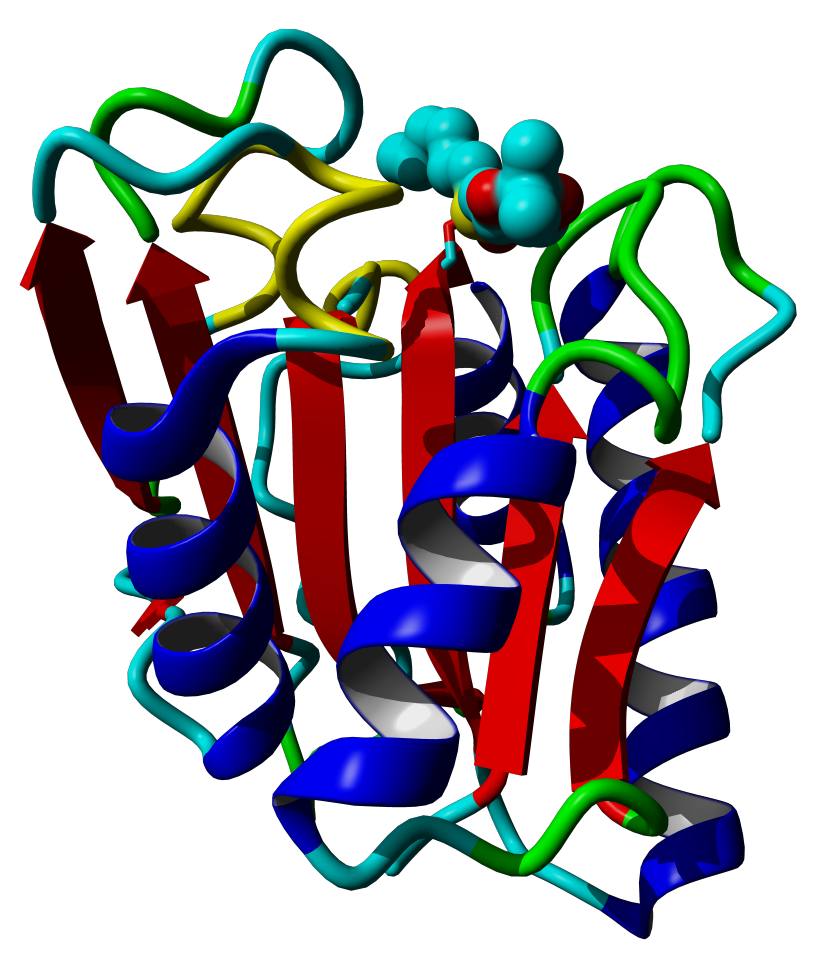
\includegraphics[width=.9\linewidth]{figures/Lipase.png}
        \end{figure}     
        \tiny Bacillus subtilis lipase A with covalently bound Rc-IPG-phosphonate inhibitor (PDB: 1R4Z)

    \end{columns} 

\end{frame}

% ============================================================================ %

\begin{frame}
    \frametitle{Proteins}
    \framesubtitle{BsLA}

    \begin{columns}[t]
        \column{.6\linewidth}
        \begin{itemize}
            \item 181 amino acids
            \item 19.3 kDa
            \item Much smaller than lipases from other organisms
            \item Active site not covered by lid but solvent exposed -- \textbf{no interfacial activation} (activation due to lid opening in presence of lipid aggregates)
            \item Very tolerant to basic pH, \textbf{optimum activity at pH 10}
        \end{itemize} 

        \column{.4\linewidth}
        \begin{figure}
            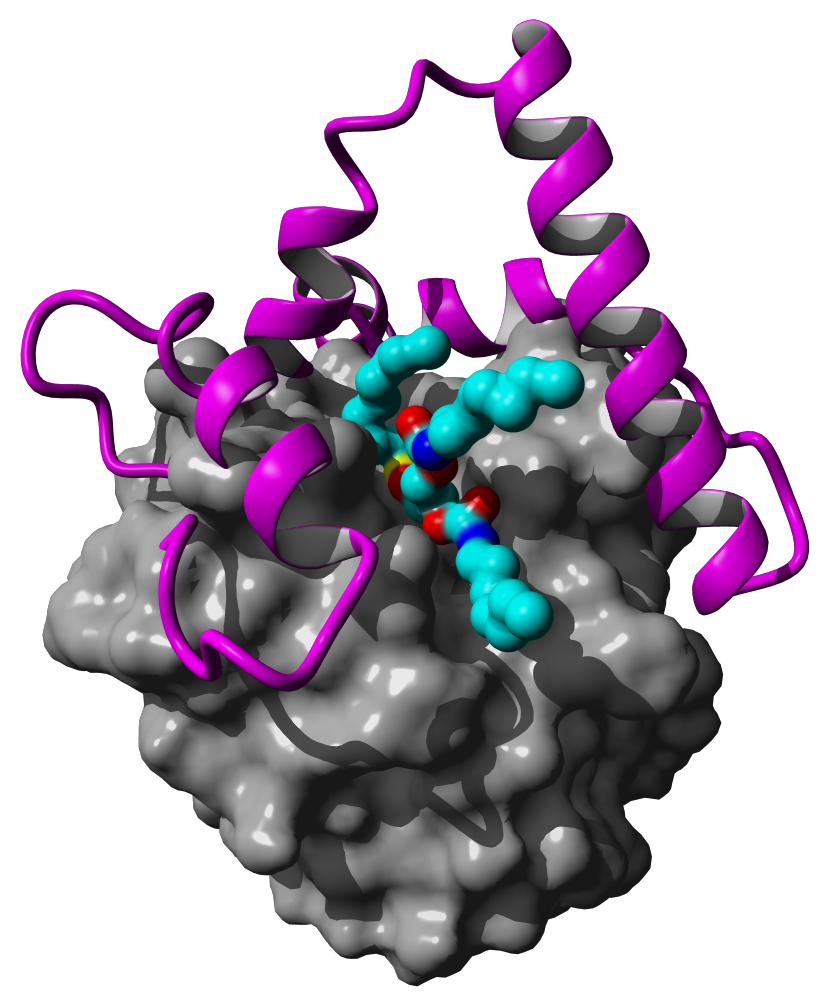
\includegraphics[width=\linewidth]{figures/Lipase_Lid.png}
        \end{figure}     
        \tiny BsLa lacks a lid covering the active site (Lid taken from P. Aeruginosa lipase, PDB: 1EX9)

    \end{columns} 

\end{frame} 

% ============================================================================ %

\begin{frame}
    \frametitle{Proteins}
    \framesubtitle{CitA-PAS}

    \begin{itemize}
        \item Part of a two component system of a sensor and a response regulator
        \item CitA: Sensor Histidine Kinase
        \item PAS: Per--Arnt--Sim domain superfamily of $\alpha/\beta$ proteins
        \item CitB: is the corresponding response regulator
        \item \textit{Klebsiella pneumoniae} two component system is essential for the induction of citrate fermentation genes in the presence of citrate
    \end{itemize}
\end{frame} 

% ============================================================================ %

\begin{frame}
    \frametitle{Proteins}
    \framesubtitle{CitA-PAS active site opening}
    \begin{figure}
        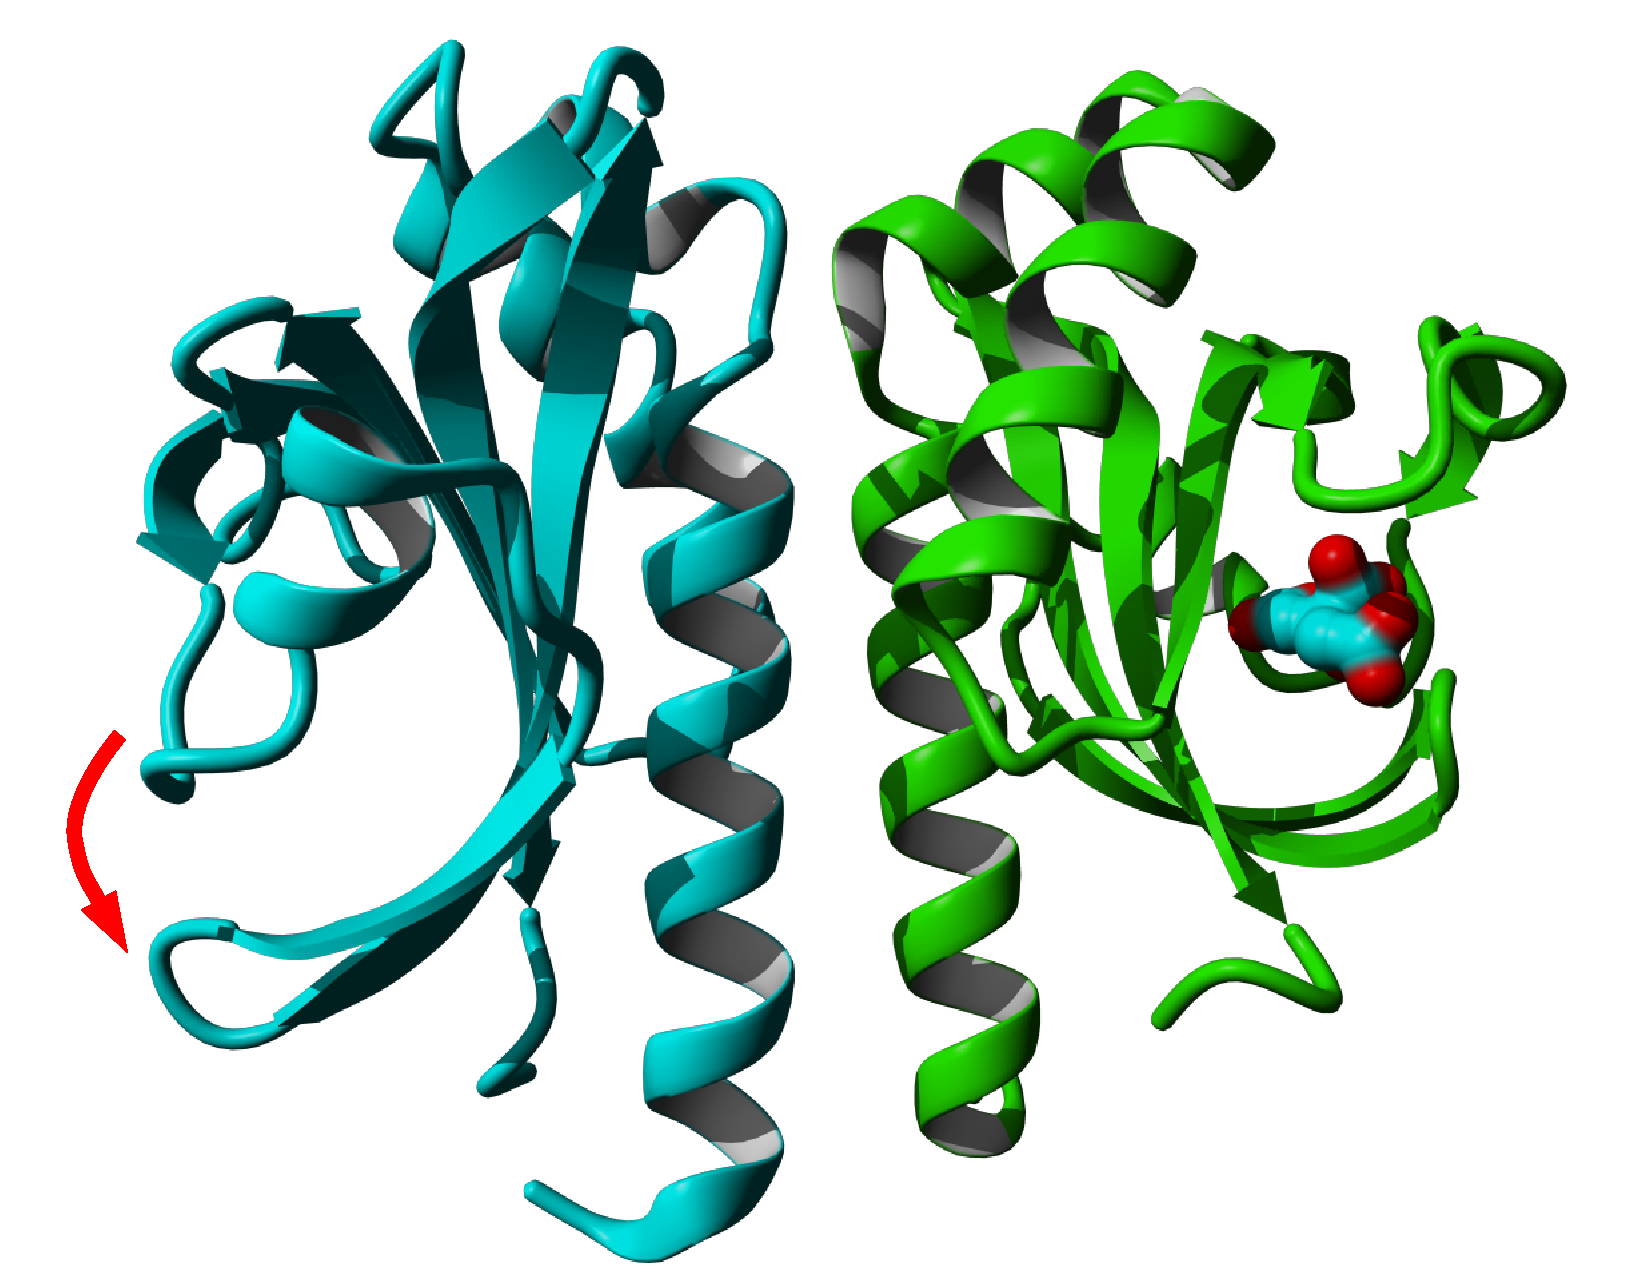
\includegraphics[width=.8\linewidth]{figures/CitA_dimer.pdf}
    \end{figure}      

\end{frame}   

% ============================================================================ %

\begin{frame}
    \frametitle{Proteins}
    \framesubtitle{CitA-PAS signal transduction mechanism}
    \begin{figure}
        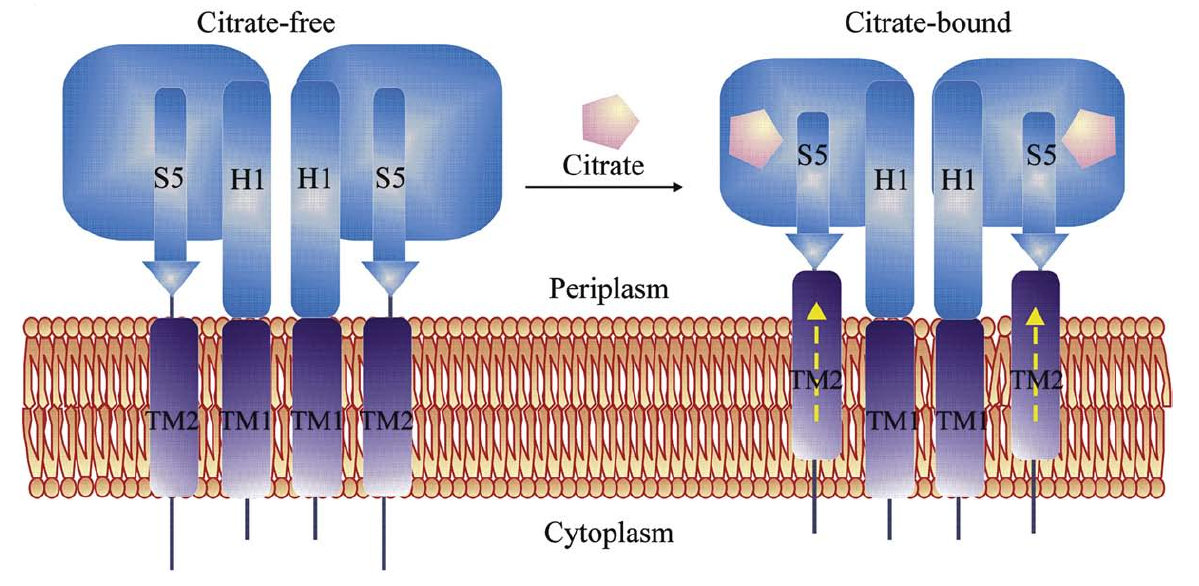
\includegraphics[width=.9\linewidth]{figures/CitA_mechanism.png}
    \end{figure}      

    \tiny
    M. Sevvana, et. al,
    \href{http://www.sciencedirect.com/science/article/pii/S0022283608000466}
    {A LIgand--Induced Switch in the Periplasmic Domain of Sensor Histidine Kinase CitA},
    \textit{J. Mol. Biol.}, 377, 512--523, 2008

\end{frame}  

% ============================================================================ %

\begin{frame}
    \frametitle{Proteins}
    \framesubtitle{Complex}

    \begin{block}{Why make a complex?}
        If citrate could trigger lipase activity we had a switchable detergent!
    \end{block}

    \pause

    \begin{columns}[t]
        \column{.88\linewidth} 
        \begin{figure}
            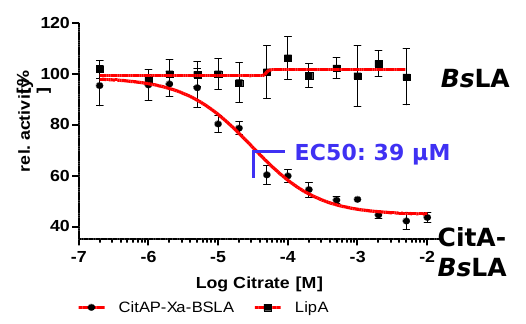
\includegraphics[width=.7\linewidth]{figures/complex/dose_response_curve.png}
        \end{figure}       

        \column{.12\linewidth} 
        \tiny
        Jaeger et al.
    \end{columns}

\end{frame}  

% ============================================================================ %

\begin{frame}
    \frametitle{Proteins}
    \framesubtitle{Complex}

    \begin{figure}
        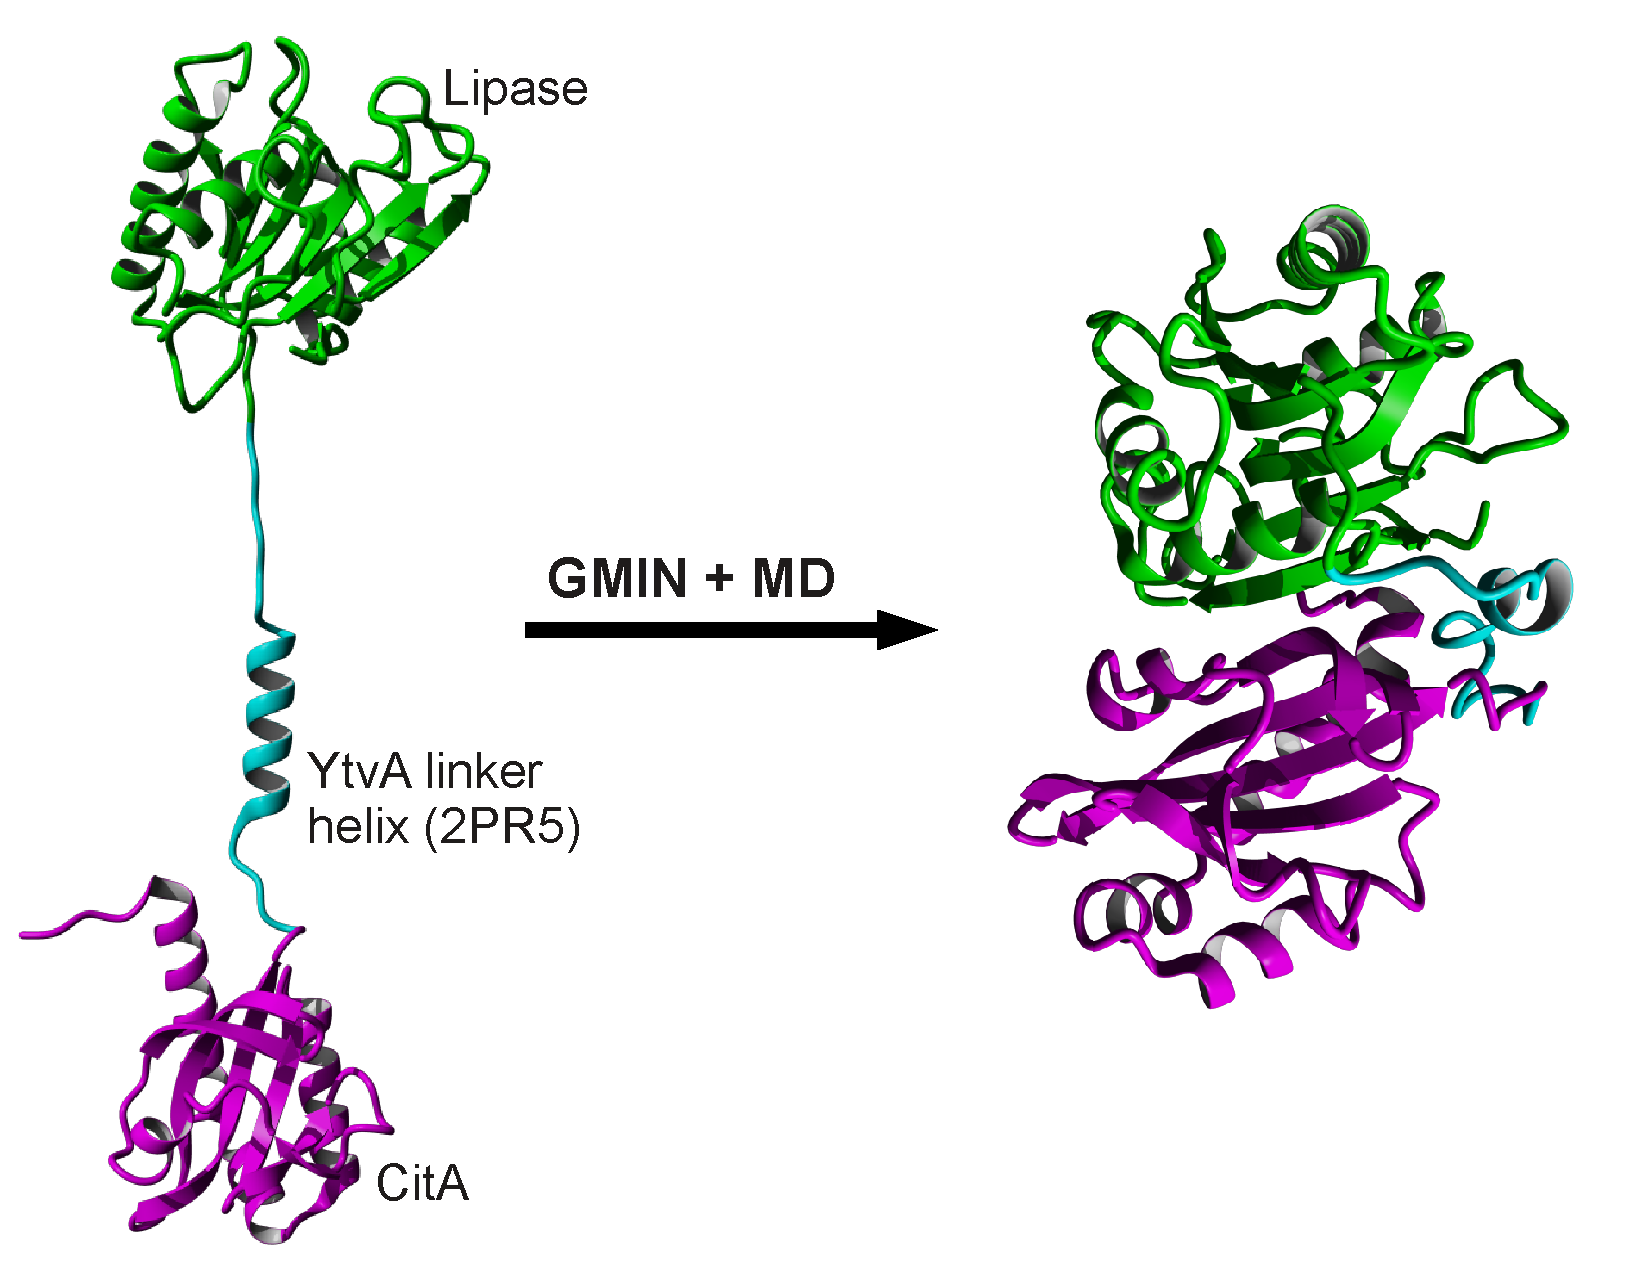
\includegraphics[width=.9\linewidth]{figures/complex/complex_folding.pdf}
    \end{figure}       

\end{frame}   

% ============================================================================ %

\section{Methods}

\begin{frame}
    \frametitle{Methods}
    \framesubtitle{Forcefield: Amber99sb-ildn-nmr}

    Uncertainty weighted objective function: $\chi^2 = \sum_i(x_i^{Exp} - x_i)^2 / \sigma_i^2$

    \begin{figure}
        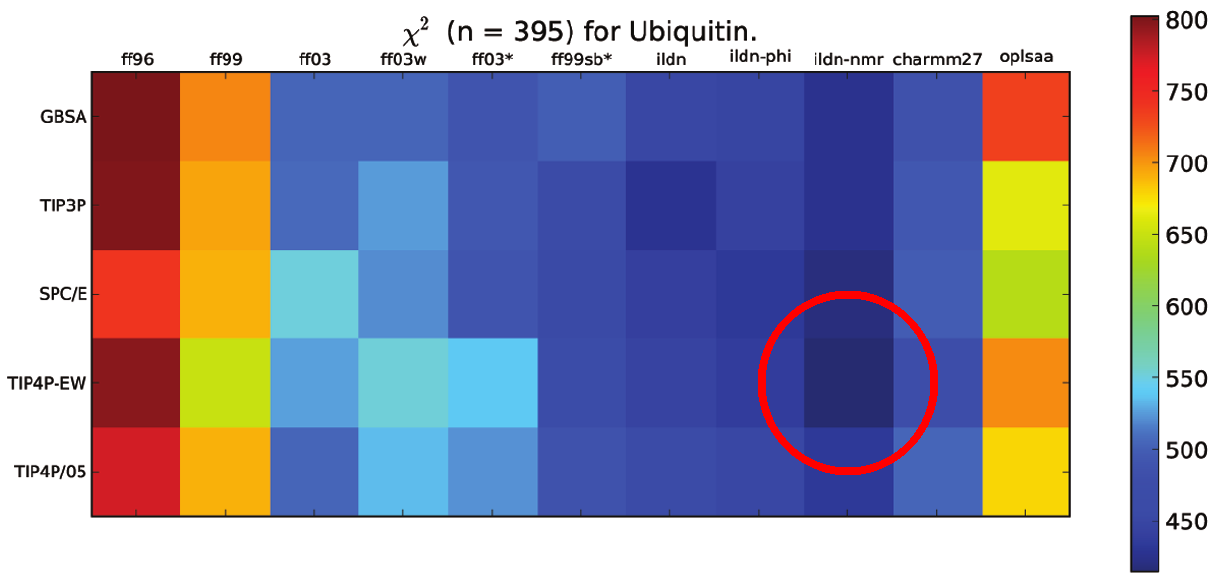
\includegraphics[width=\linewidth]{figures/forcefield_performance.png}
    \end{figure}        

    \tiny
    K. A. Beauchamp, Y. Lin, R. Das and V. S. Pande,
    \href{http://pubs.acs.org/doi/abs/10.1021/ct2007814}
    {Are Protein Force Fields Getting Better?
    A Systematic Benchmark on 524 Diverse NMR Measurements},
    \textit{J. Chem. Theory Comput.},
    8, 1409--1414, 2012
    

\end{frame}   

% ============================================================================ %

\begin{frame}
    \frametitle{Methods}
    \framesubtitle{Citrate Forcefield Parameterization}

    \begin{figure}
        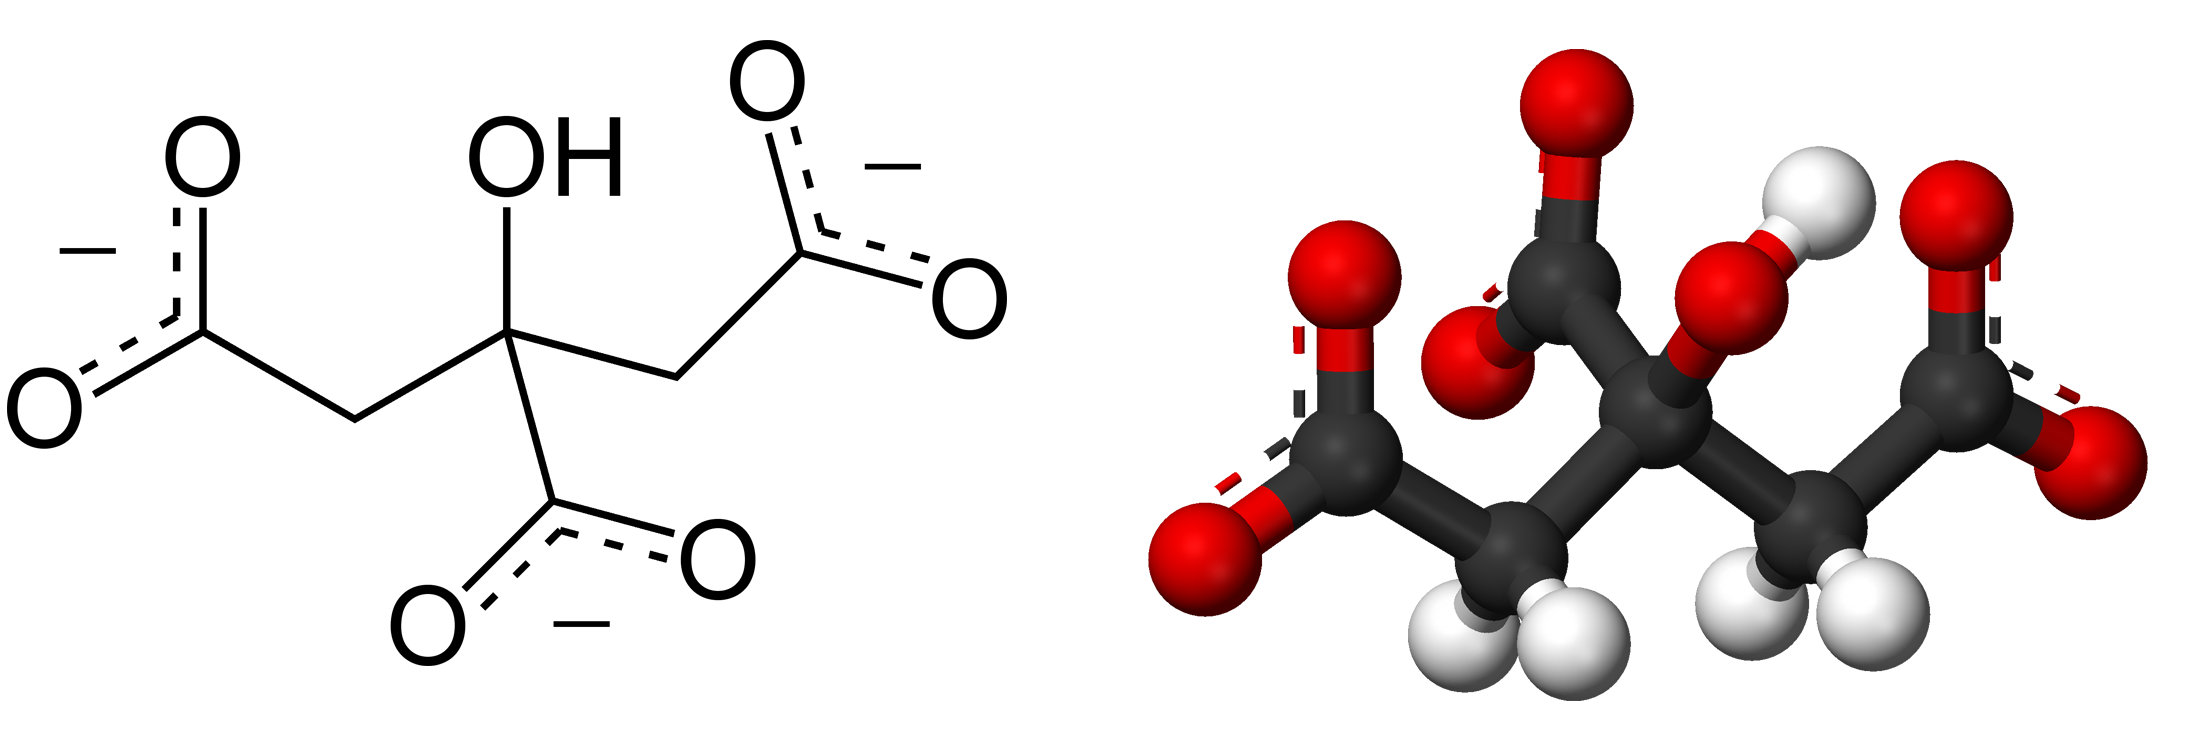
\includegraphics[width=.7\linewidth]{figures/citrate.png}
    \end{figure}      

    \begin{itemize}
        \item Parameterized with the general AMBER force field (GAFF) from Ambertools
        \item Partial charges come from
        \begin{itemize}
            \item \textbf{Antechamber} -- AM1-BCC (parameterized fit to \textit{ab initio} calculations)
            \item YASARA AutoSIMLES Server -- ''improved'' AM1-BCC
            \item \textit{ab initio}
        \end{itemize}
    \end{itemize}
\end{frame}   
 
% ============================================================================ %

\begin{frame}
    \frametitle{Methods}
    \framesubtitle{pKa Prediction} 

    \begin{block}{Why different pH?}
        \begin{itemize}
            \item Optimum activity at pH 10
            \item Activity measurements shown performed at pH 7.5
            \item Other experiments (fluorescence) at pH 10
            \item Highest CitA--citrate affinity at pH 5.5
        \end{itemize}
    \end{block}

    \pause
    \vspace{0.5cm}

    \center
    $\Longrightarrow$ Protonation states at different pH \\
    $\Longrightarrow$ WANTED: reliable pKa predictions

\end{frame}

% ============================================================================ %

\begin{frame}
    \frametitle{Methods}
    \framesubtitle{pKa Prediction} 

    Different Methods for pKa prediction (expensive)
    \begin{itemize}
        \item Continuum electrostatics based on
        \begin{itemize}
            \item linearized Poisson--Boltzmann equation (\textbf{MEAD})
            \item Generalized--Born approximation
            \item Multiple rotamers can be considered in a Monte--Carlo approach (\textbf{MCCE})
        \end{itemize}

        \item empirical Methods (including rotamers) (\textbf{PROPKA})
    \end{itemize}

    \pause

    \begin{center}
    \begin{tabular}{ c c c c }
         & \multicolumn{3}{c}{\% predictions} \\
        $|pKa_{pred} - pKa_{exp}|$ & MEAD & MCCE & PROPKA \\
        \hline
        \hline
        <2   & 66.7 & 76.9 & \textbf{87.2} \\
        <1.5 & 48.7 & 64.1 & \textbf{82.1} \\
        <1   & 25.6 & 43.6 & \textbf{66.7} \\
        <0.5 & 15.4 & 20.1 & \textbf{35.9} \\
    \end{tabular}
    \end{center}

\end{frame}

% ============================================================================ %

\begin{frame}
    \frametitle{Methods}
    \framesubtitle{pKa Prediction} 

    \begin{equation*}
        \frac{[A]}{[AH]} = 10^{pH - pKa}
    \end{equation*} 

    \begin{center}
    \begin{tabular}{ c c c c }
         & \multicolumn{3}{c}{\% predictions} \\
        $|pKa_{pred} - pKa_{exp}|$ & MEAD & MCCE & PROPKA \\
        \hline
        \hline
        <2   & 66.7 & 76.9 & \textbf{87.2} \\
        <1.5 & 48.7 & 64.1 & \textbf{82.1} \\
        <1   & 25.6 & 43.6 & \textbf{66.7} \\
        <0.5 & 15.4 & 20.1 & \textbf{35.9} \\
    \end{tabular}
    \end{center}

    \tiny
    M. N. Davies, C. P. Toseland, D. S. Moss and D. R. Flower,
    \href{http://www.biomedcentral.com/1471-2091/7/18/}
    {Benchmarking pKa prediction},
    BMC Biochemistry, 7(18), 2006

\end{frame}
 
 
% ============================================================================ %

\section{Results}

\begin{frame}
    \frametitle{Results}
    \framesubtitle{CitA-PAS Binding Pocket}

    \begin{figure}
        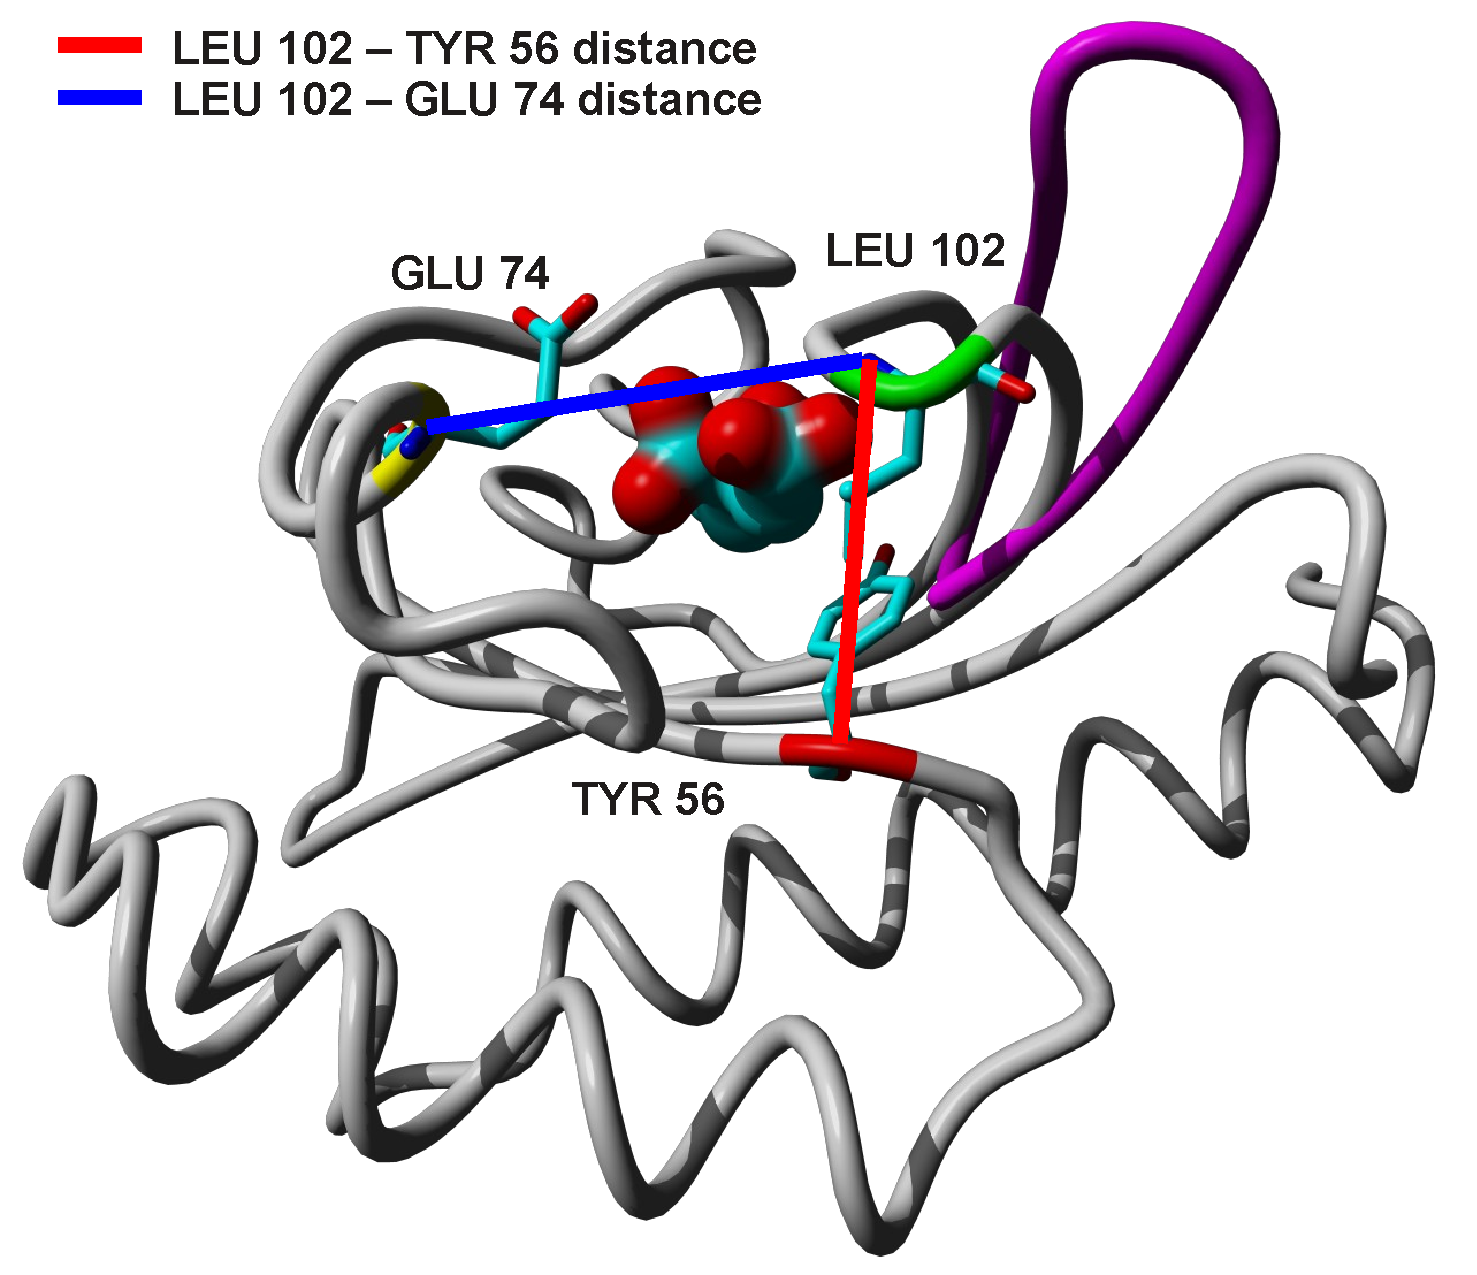
\includegraphics[width=.7\linewidth]{figures/CitA_pocket2.pdf}
    \end{figure}     
\end{frame}    

% ============================================================================ %

\begin{frame}
    \frametitle{Results}
    \framesubtitle{CitA-PAS Citrate free}

    \begin{figure}
        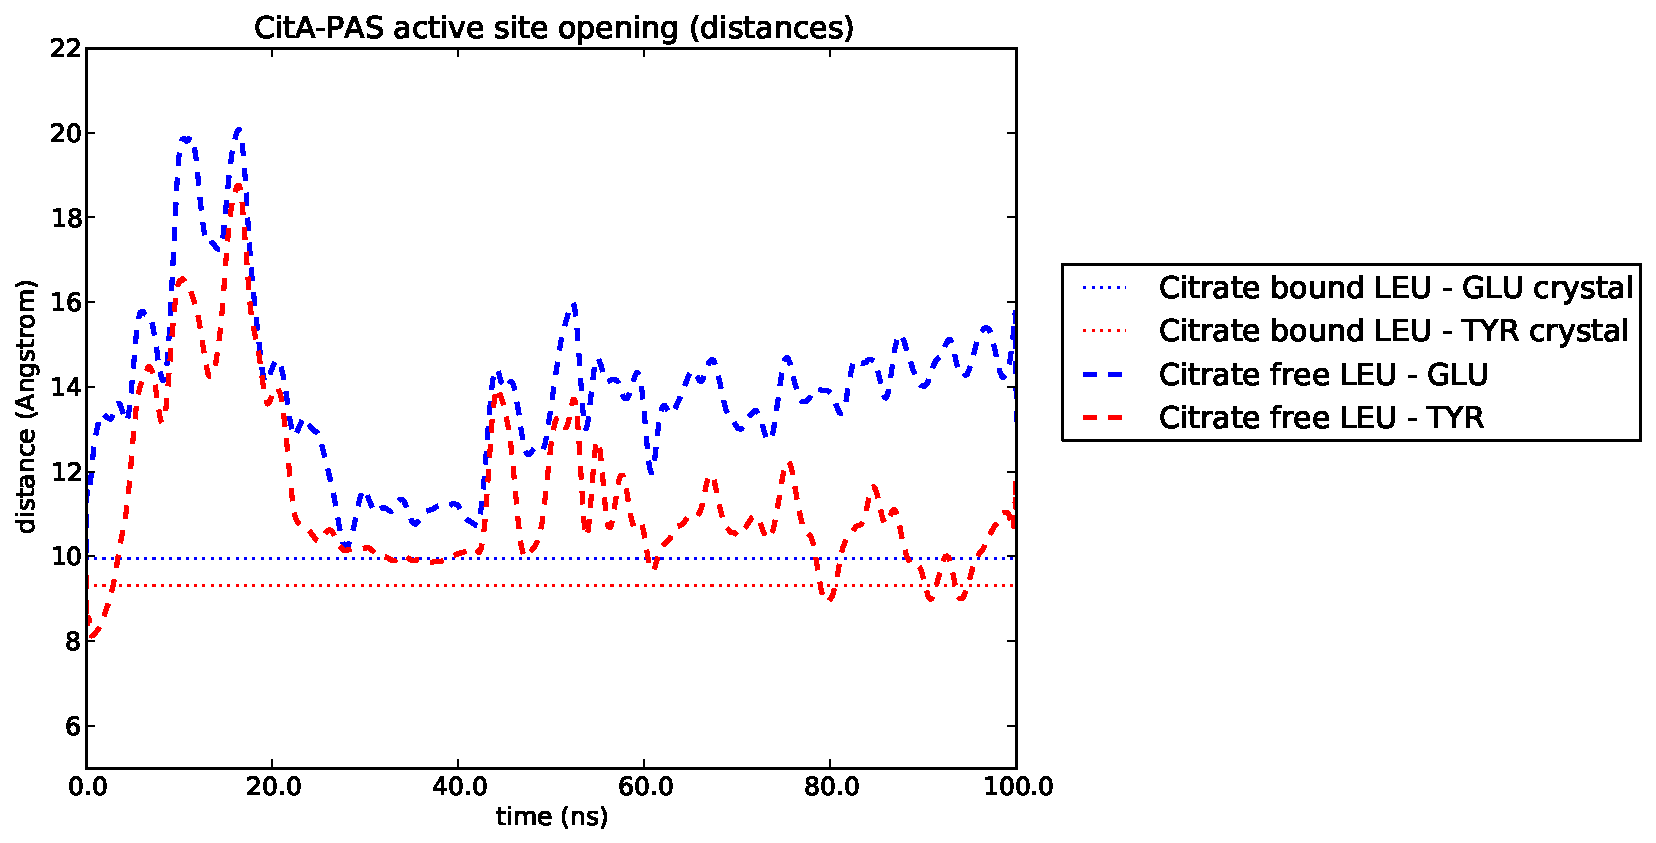
\includegraphics[width=1.05\linewidth]{figures/MD/distances_citrate_free.pdf}
    \end{figure}      
\end{frame}   
 

% ============================================================================ %

\begin{frame}
    \frametitle{Results}
    \framesubtitle{CitA-PAS Citrate free and bound}

    \begin{figure}
        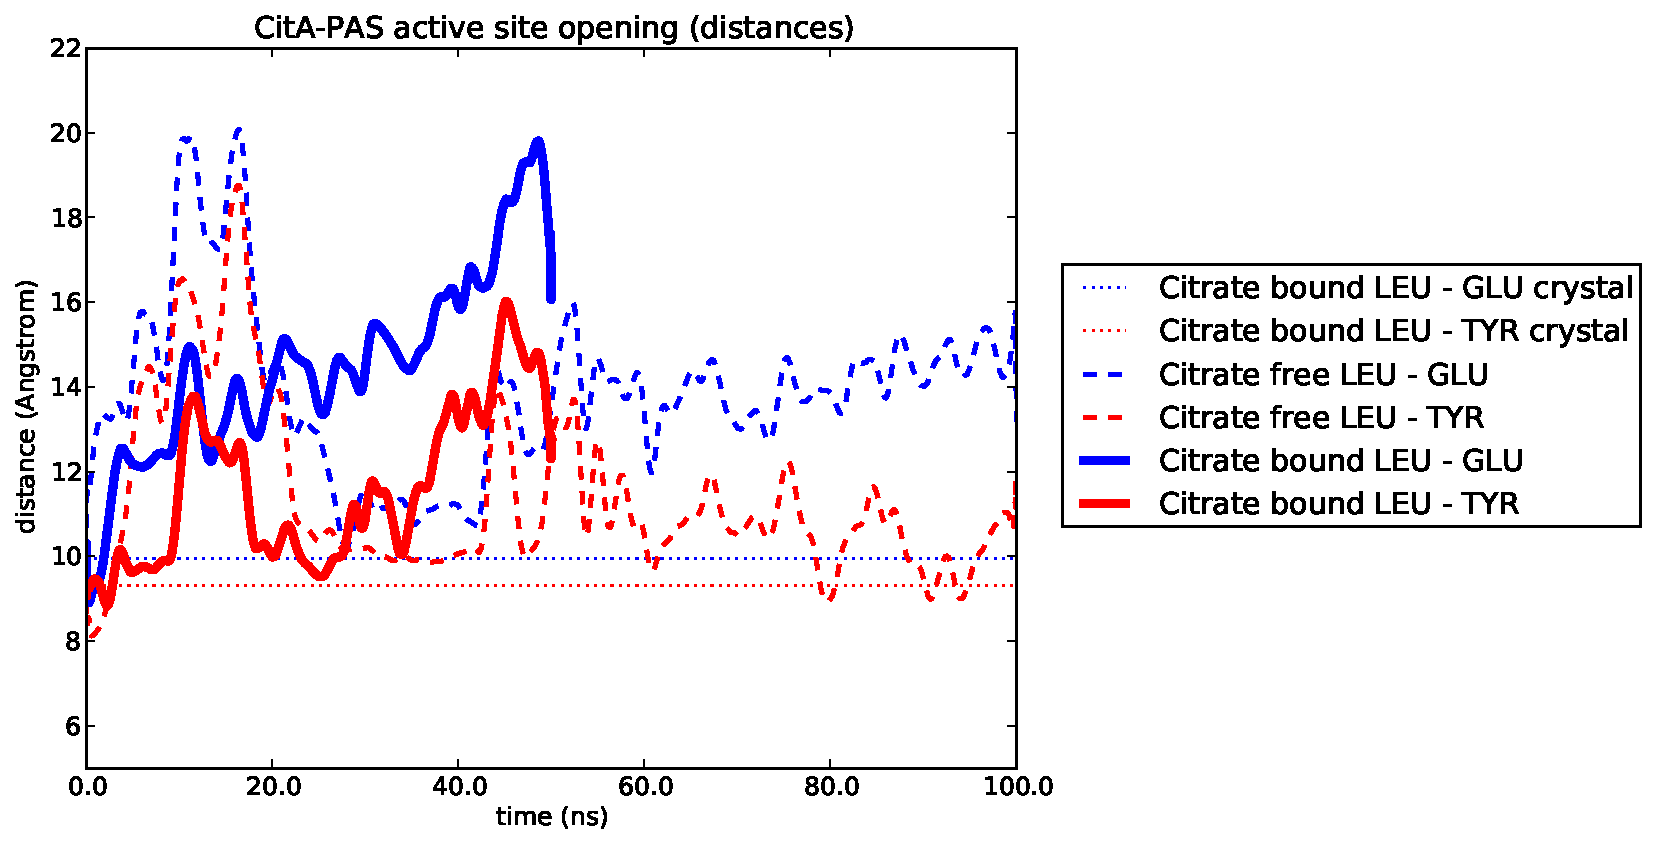
\includegraphics[width=1.05\linewidth]{figures/MD/distances_both.pdf}
    \end{figure}      
\end{frame}   
 
% ============================================================================ %

\begin{frame}
    \frametitle{Results}
    \framesubtitle{CitA-PAS Citrate free}

    \begin{figure}
        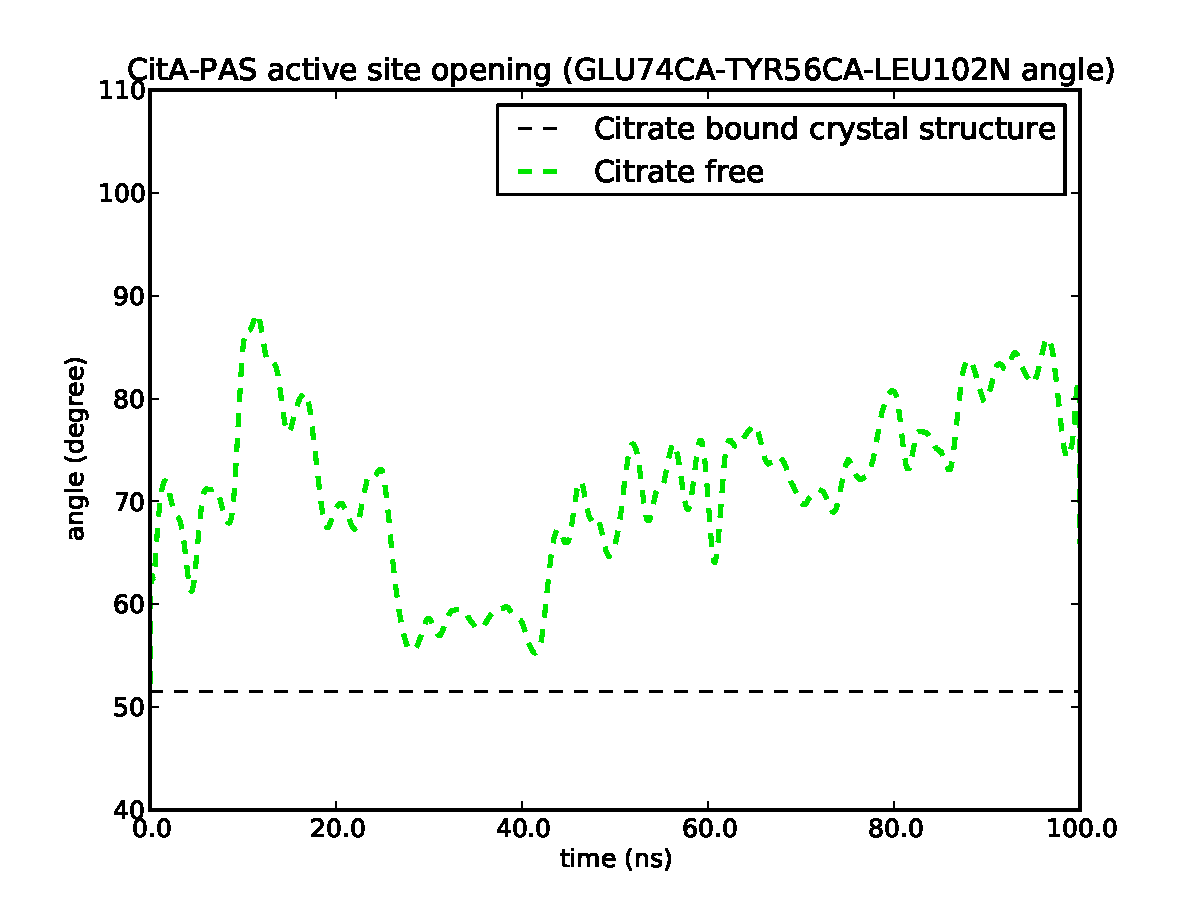
\includegraphics[width=.85\linewidth]{figures/MD/angle_citrate_free_GLU74CA-TYR56CA-LEU102N.pdf}
    \end{figure}       
\end{frame}   
 
% ============================================================================ %

\begin{frame}
    \frametitle{Results}
    \framesubtitle{CitA-PAS Citrate free and bound}

    \begin{figure}
        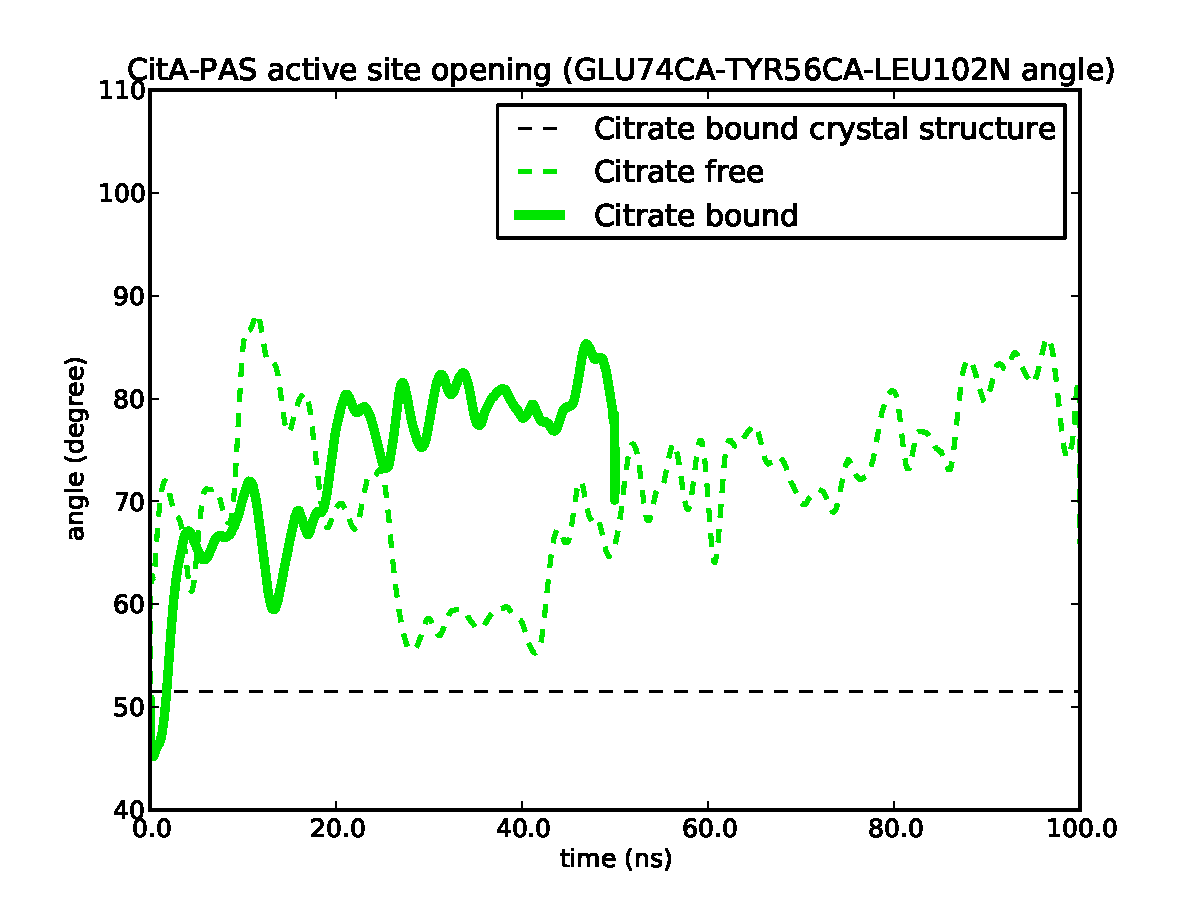
\includegraphics[width=.85\linewidth]{figures/MD/angle_both_GLU74CA-TYR56CA-LEU102N.pdf}
    \end{figure}       
\end{frame}   
 
% ============================================================================ %

\section{Outlook}

\begin{frame}
    \frametitle{Outlook}
    \framesubtitle{Future Plans}

    \begin{itemize}
        \item Validate citrate bound \textbf{CitA opening} at different pH
        \item Check \textbf{BsLA stability} at different pH
        \item Generate more CitA--BsLA complex structures (GMIN)
        \item \textbf{Simulate complex} at different pH

        \pause

        \item Compare complex to experiment
            \begin{itemize}
                \item \textbf{SAXS} (timescale: \textasciitilde Month)
                \item \textbf{X--ray} structure (timescale: Masterthesis)
                \item \textbf{NMR} (timescale: PhD Thesis)
                \item Tryptophan / Tyrosine \textbf{fluorescence}
            \end{itemize}

        \pause

    \item Elucidating the mechanism of lipase activation by \textbf{nonequilibrium MD}
    \end{itemize}
\end{frame}   
 
% ============================================================================ %

\end{document}
